\Chapter{Beam Line Design}%________________________________
\Section{Kicker Design}

As described in Chapters 2, a fast rise time kicker is needed to separate the 
bunch trains supplied by the drive line. The spacing between bunch trains is on the 
order of nanoseconds, and depends on the layout of the beam lines and laser timing.
Magnetic options, such as a dipole, were disqualified due to their slow rise times 
(on the order of seconds). \nrnote{is that right? Might be miliseconds? neet to find source for this}
Therefore an electrostatic approach was chosen, due to achieve faster rise times.

Borrowing from a successful neighbor, a design implemented by Indiana University (IU) \cite{iukicker}
was adapted to fit the TBA requirements at the AWA. Redesign required consideration
of the length and gap between the kicker plates. Both are key parameters that determine 
what angle the beam will be deflected. Longer plates results in the beam traveling 
in the electromagnetic field for a longer amount of time (i.e. larger angle). 
A smaller gap increase the field intensity for a give voltage, consider a parallel plate 
capacitor and Guass' law. This can also increase the angle.


The kicker is essentially a parallel plate waveguide. 
A $\pm$\SI{30}{kV} power supply will be used to induce a maximum of \SI{60}{kV} potential difference 
across the plates. Each plate will be terminated in a 50 $\Omega$ load to induce a steady 
state current on the plates. The combination of the two plates will result in a static TEM mode 
between the plates. Calculation of the electric, $E_v$, and magnetic field, $B_v$,
can be derived from the voltage or current. The electric field, $E_v$, due to a potential, V, is: 
\begin{equation}
E_v=\frac{V}{h}
\end{equation}

Where h is the gap height. From Maxwell's equations, we know that the electric and magnetic 
field are related by the speed of light, c, in the case of plane and TEM waves \cite{pozar}. 
From this we can find the magnetic field induced between the plates: 
\begin{equation}
B_v=\frac{E_v}{c}
\end{equation}\label{Bv}
The electrons are traveling at nearly the speed of light, $c$, and move through the kicker on a 
trajectory perpendicular to the fields.  Plugging Equation \ref{Bv} into the Lorentz force equation, 
it is shown that the force exerted on a charge, q, 
from the electric and magnetic fields of the TEM mode are equal. 
\begin{equation}
F=q\,(E_v+v\times B_v)
\end{equation}
\begin{equation}
	F = q \,\left(E_v+c\times \frac{E_v}{c}\right)
\end{equation}

Since the force due to the electric field is equal and oriented in the same direction as the field due to the magnetic field, 
the total kick is twice that from either field alone.  
The angle induced by electric and magnetic fields has been calculated in \cite{iukicker, Wiedemann}
and is rewritten in the following terms:  
\begin{equation}
\theta_E= \frac{V\,L}{h\,T}
\end{equation}
\begin{equation}
\theta_B= \frac{B\,L}{B\rho}
\end{equation}

Where L is the plate length, and T is the kinetic energy of the beam. 
Rigidity, or $B\rho$, is a common accelerator physics term that can be found in text such as Wiedemann \cite{Wiedemann}. 
It is a convenient way to relate the magnetic field and trajectory of an energetic beam traveling through that field.
\begin{equation}
	B\rho=3.33564\,*T\, \text{[GeV-Tesla]}
\end{equation} 
Using the definitions above, the total angle provided by the kicker is then: 
\begin{equation}
\theta_{total}= \theta_E+\theta_B=2\theta_E=2\theta_B
\end{equation}
From these equations, design parameters include the gap height, length of the plates, and 
the kinetic energy of the beam. The largest drive beam energy achievable at the AWA is 75 MeV. 
With this in mind, T was set as a constant, and the gap and length of the plates were adjusted.
Simulations in 
\begin{figure}[h]
	\begin{center}
		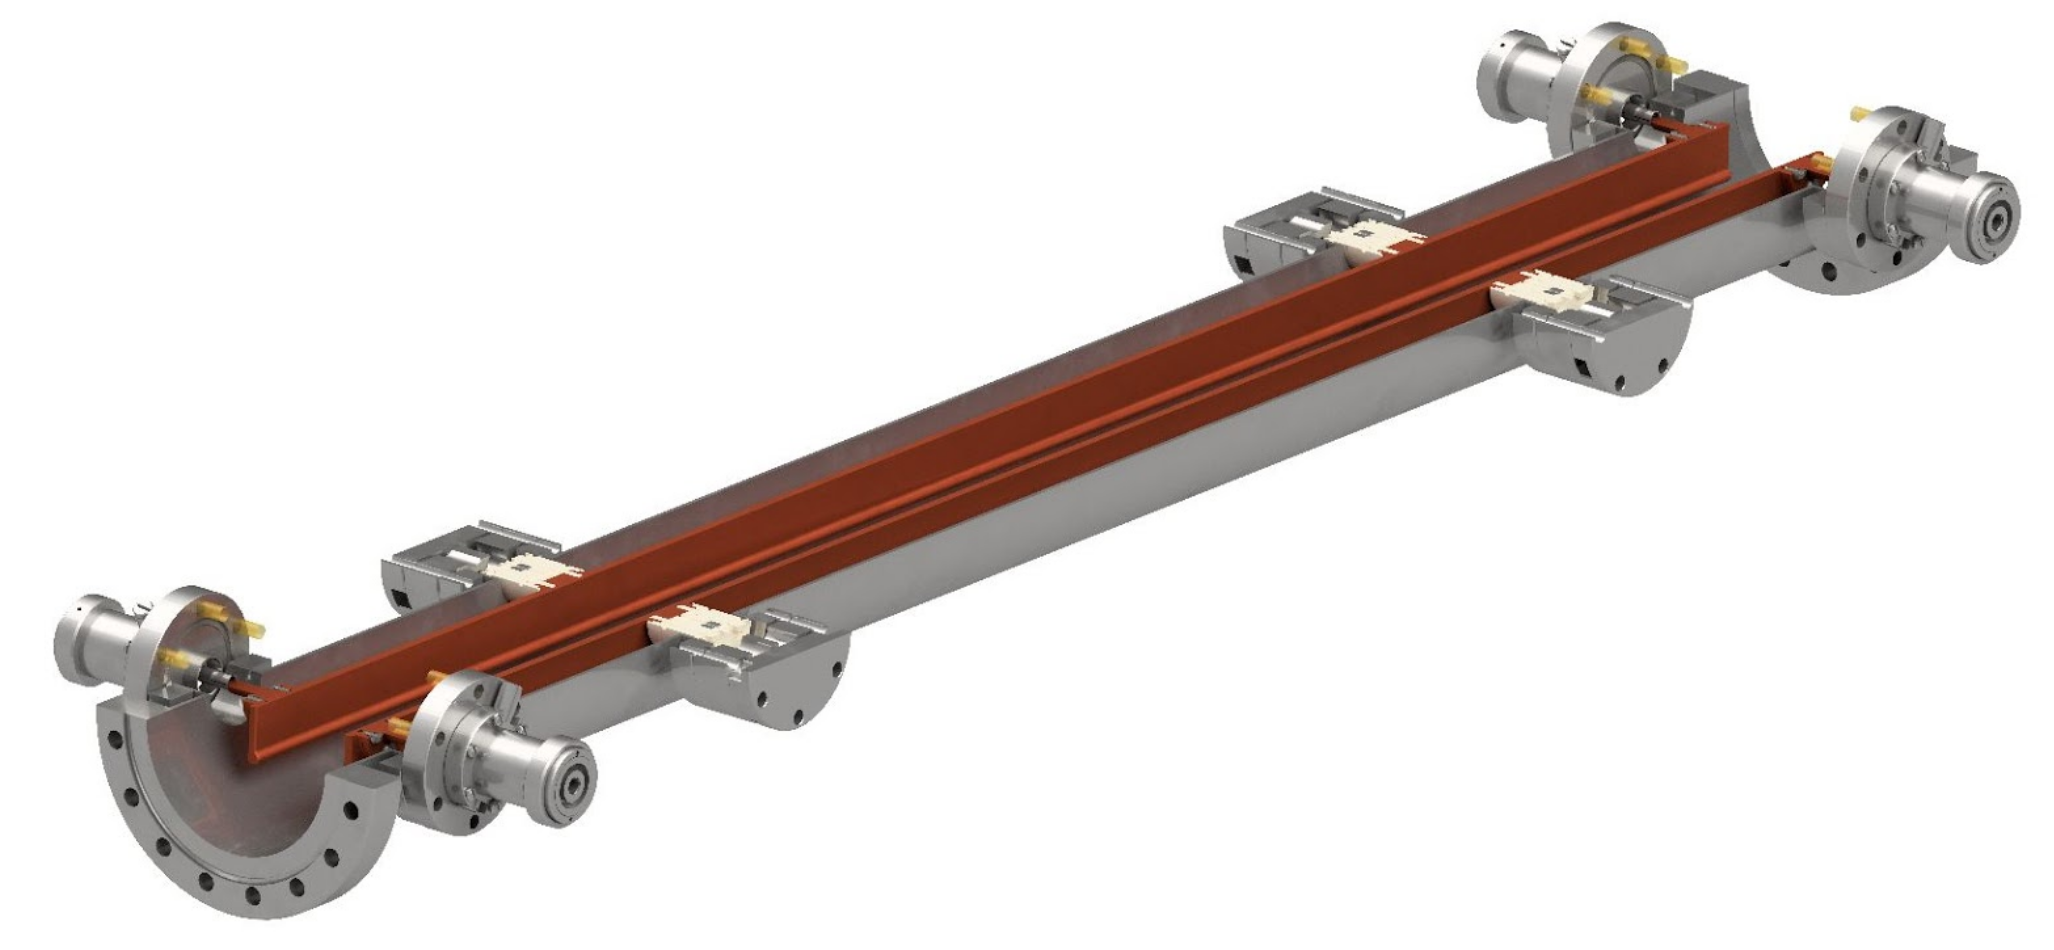
\includegraphics[width=0.75\textwidth]{./images/kicker}\caption{CAD drawing of AWA kicker design }
		\label{fig:AWAkicker}
	\end{center}
\end{figure}

However there are other limitations to consider. The gap needs to be large enough 
to allow the full width of the beam to pass through while it is being deflected.


\Subsection{CST Results??}
\nrnote{Jiaqi from Euclid did a quick check of the design in CST. I have some plots from him, but none of the original data.
I wouldn't be able to re plot this work...not sure if I should include this.}

\Section{Outside Vacuum Kicker Tests}

After the design of the kicker was finalized, fabrication began at ANL.
The copper plates and ceramic brackets were fabricated on site at the ANL shops.
High voltage (HV) feedthroughs and cables were purchased from FID GmbH. 
In order to test that the fabrication of the kicker was sound, members of the 
Advanced Photon Source (APS) electronics groups graciously helped perform an 
out of vacuum AC high voltage test. Afterwards they also helped perform and 
analyze a TDR measurement of the kicker plates.
\begin{figure}[h]
	\begin{center}
		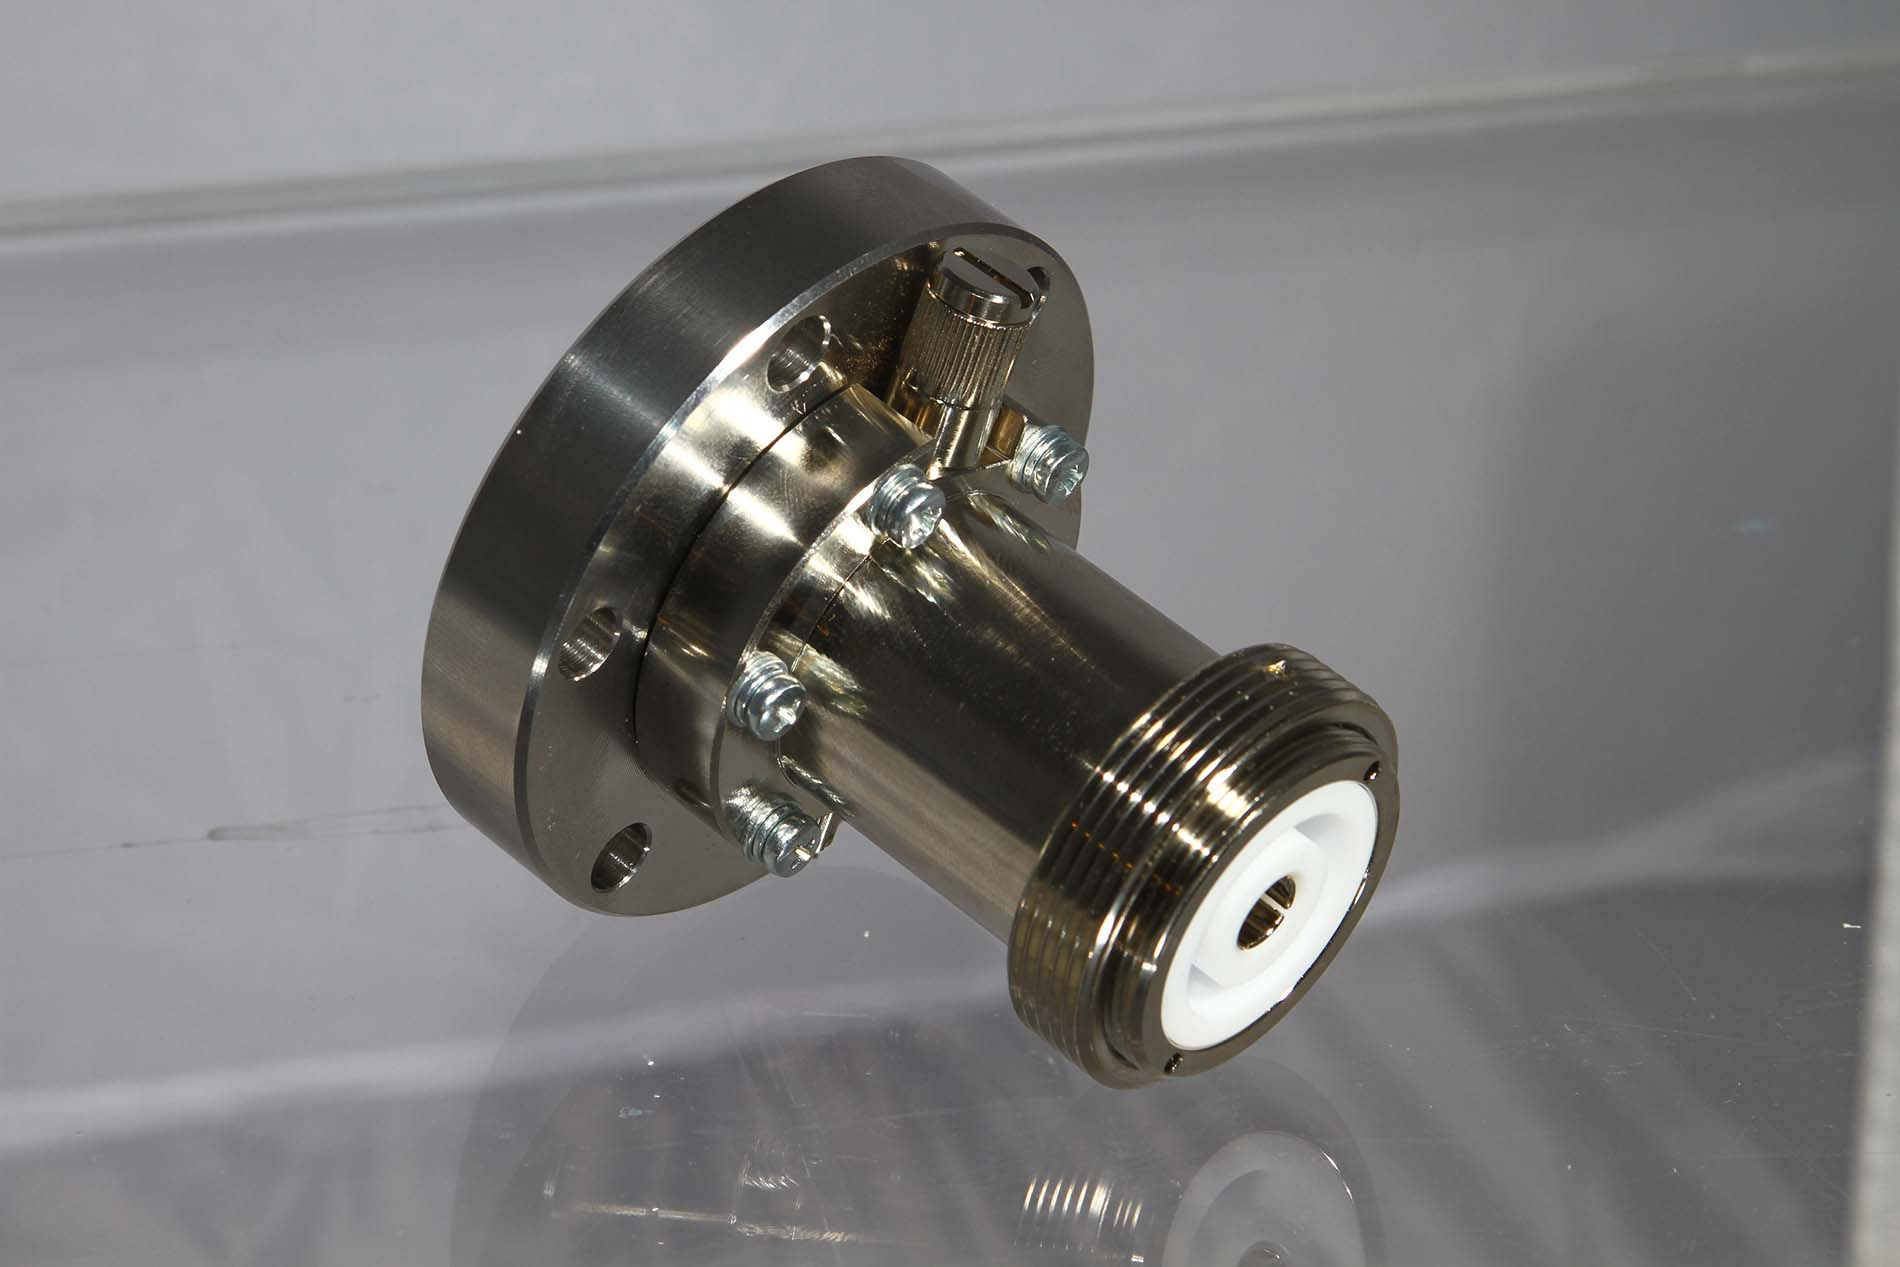
\includegraphics[width=0.5\textwidth]{./images/FID_feedthrough1}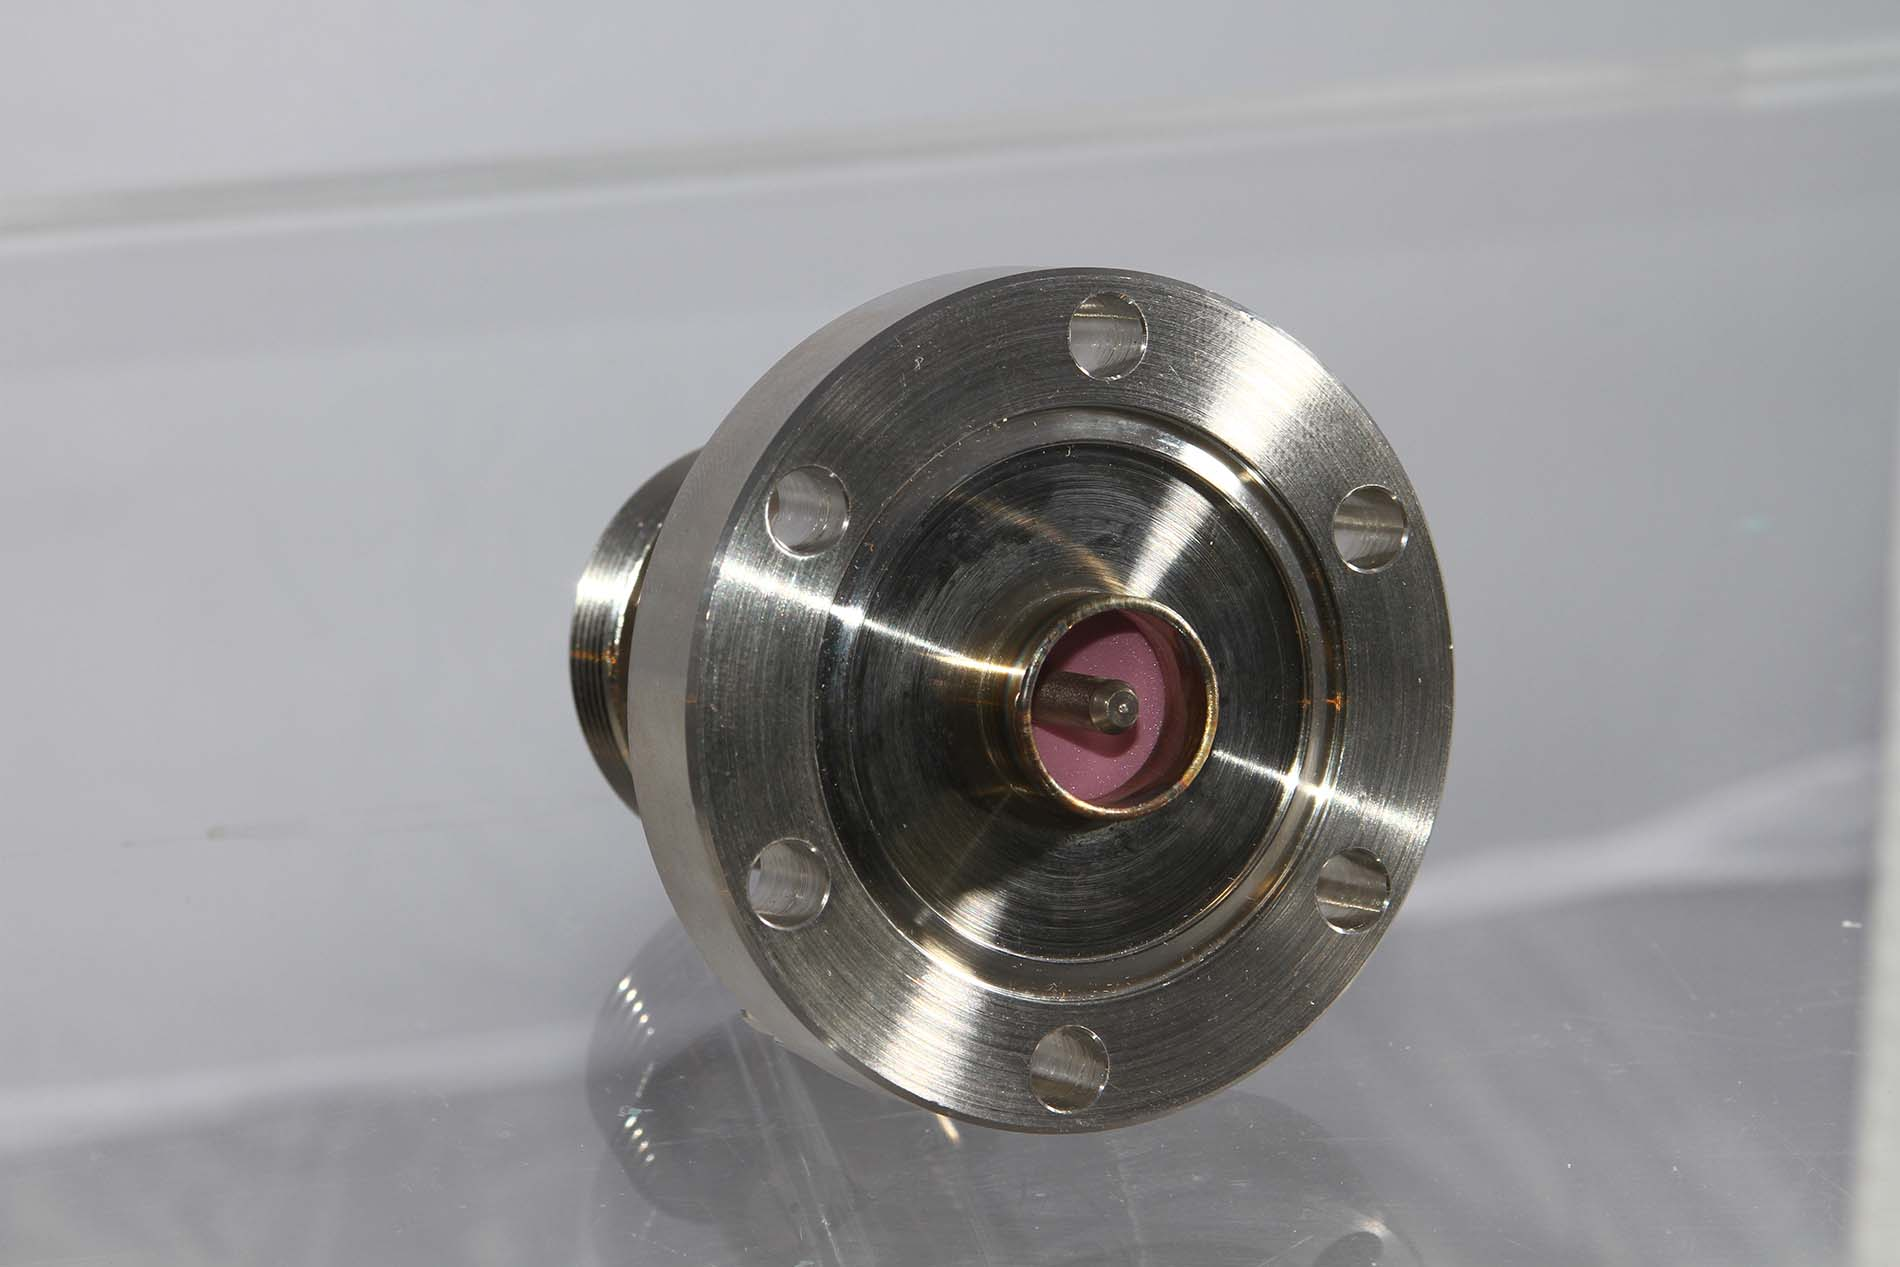
\includegraphics[width=0.5\textwidth]{./images/FID_feedthrough2}
		\caption{High voltage feedthrough purchased from FID GmbH. Left, connection to the HV cables.
		Right, is the in vacuum pin that connects to the copper kicker plates.}
		\label{fig:feedthroughs}
	\end{center}
\end{figure}


\Subsection{High Voltage Test}

Two HV tests were performed at the APS. 
The first test consisted of HV applied in increments to ports 3 and 4 on the kicker.
Ports 1 and 2 were shorted to ground. There was no leakage current up to \SI{8}{kV} RMS.
The second test reversed the set up with 3 and 4 grounded and ports 1 and 2 exposed. 
There was no leakage current up to \SI{9}{kV} RMS, which was the maximum voltage of the test equipment.
Figure~\ref{fig:AWAHVkicker} shows the connection and location of the kicker in the APS Faraday cage.

\begin{figure}[h]
	\begin{center}
		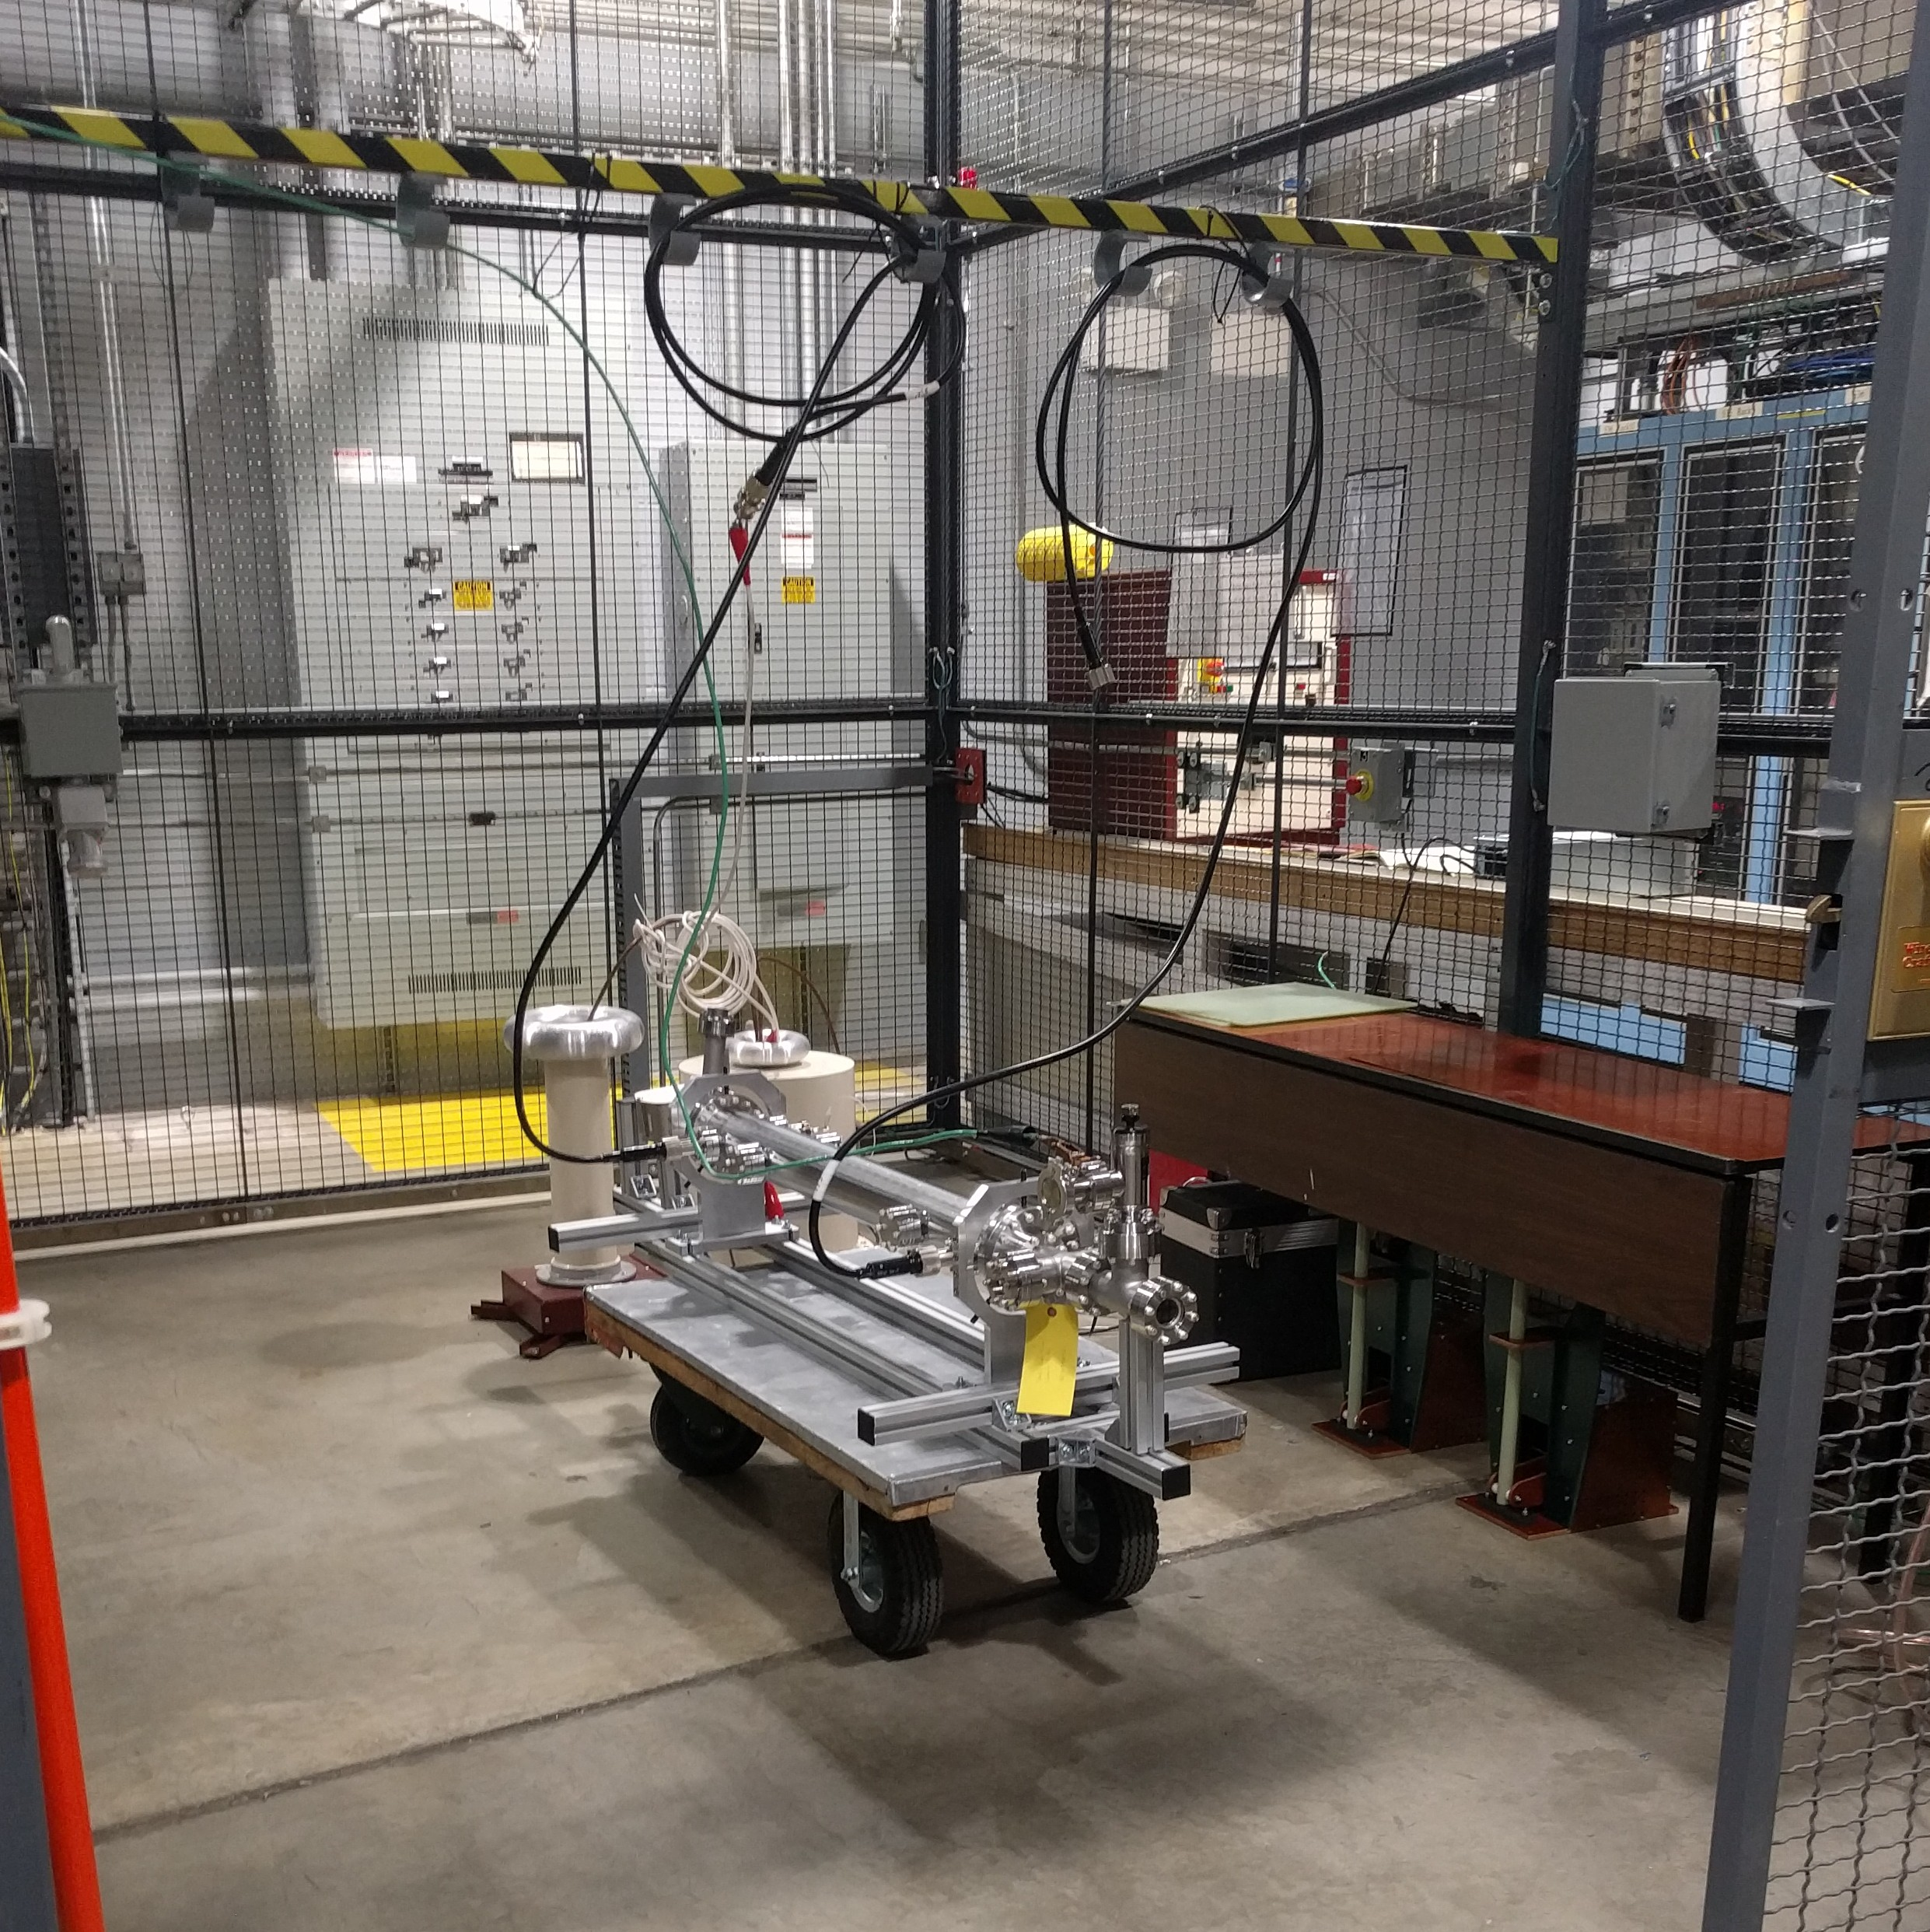
\includegraphics[width=0.7\textwidth]{./images/kicker1}\caption{High voltage set up at the APS. The kicker was grounded on one side and exposed to HV AC power on the other. The Faraday cage was closed during testing. }
		\label{fig:AWAHVkicker}
	\end{center}
\end{figure}


\Subsection{TDR Test}


\Section{Measurment of Beam Deflection}

Next the kicker was installed in the AWA drive beam line.
It's approximate location is 16.5 meters downstream of the cathode.
The HV pulsar was located on the roof of the bunker.



\Section{Matrix Formalism For TBA Beam Line}

A drift: 
\begin{equation}
R_d = 
\begin{bmatrix}
1 & L \\
0 & 1
\end{bmatrix}
\end{equation}

A quad: 
\begin{equation}
R_q = 
\begin{bmatrix}
1 & 0 \\
\pm \frac{1}{f} & 1
\end{bmatrix}
\end{equation}

A dipole:
\begin{equation}
R_s = 
\begin{bmatrix}
a & b \\
c & d
\end{bmatrix}
\end{equation}

To convert from focal length to quadrupole strength we must take into account the 
beam energy as well as the dimensions of the quadrupole. 
\begin{equation}
	\frac{1}{f} = kl \\
\end{equation}
Where $l$ is the quadrupole's effective length, and k is the gradient w.r.t 
the beam energy and magnet strength \cite{Wiedemann}:
\begin{equation}
	k = \SI{0.2998}{} \frac{g[\SI{}{T/m}]}{p [\SI{}{GeV/c}]}\label{k}
\end{equation}



 To reduce the number of free parameters quickly without using expensive PIC simulations, 
 the transfer matrix of the beam line was considered. Starting at the end of the linac, 
 we consider the first four quadrupoles before the kicker. All the quadruple strengths (4) and
 distances between the quadrupoles (6) are parameters under consideration. To reduce the number
 of variables from 10 to 4, we use the quadruplet telescope module as described by K. Brown in \cite{brown}.  The transfer matrix R, is reduced to:  
 \begin{equation}
 R_q = R_{d4} \cdot R_{q3} \cdot R_{d3} \cdot R_{q2} \cdot R_{d2} \cdot R_{q1} \cdot R_{d1} = 
 \begin{bmatrix}
 \frac{f_2 f_4}{f_1 f_3} & 0 \\
 0 & \frac{f_1 f_3}{f_2 f_4}	
 \end{bmatrix}\label{kb1}
 \end{equation}

\nrnote{add detail about this matrix comes from and expand matrix to x and y}
Where $f_1 \ldots f_4$ stand for the focal lengths of each quad before the kicker. 
Due to other experiments in the AWA tunnel, 
the first quadrupole was required to be at least $\SI{3}{m}$ away from the exit of the 
last accelerating cavity in the linac. This gives the initial drift length and value
for $f_1$. 

\Subsection{Point to Point Configuration}
To achieve point to point transport of the beam, we can 
equate $f_1 = f_4$ and $f_2 = f_3$. This reduces Eq. \ref{kb1} to:
 \begin{equation}
R_q =
\begin{bmatrix}
1 & 0 \\
0 & 1	
\end{bmatrix}
\end{equation}
We can further simplify the experimental set up by 
assuming $f_1=f_2$. Given the total distance, D, available for the
quads in the beam line, \SI{3.8}{m}, we can then solve
for the focal length $f_1$: 
\begin{align}
	D = 4f_1 + 4 f_2 = 8f_1 = \SI{3.8}{m} \\
	f_1 = \SI{0.475}{m}
\end{align}
Given an energy of \SI{65}{MeV}, a quadrupole length of \SI{11}{cm}, 
and Eq. \ref{k} we can calculate this configuration would require a 
magnet strength of \SI{4.14}{[T/m]}. This is feasible considering the 
max strength is \SI{9}{[T/m]}.

To determine the effect of this configuration on the beam size and divergence
we compare the sigma matrix before and after the qudrupoles:
\begin{align}
	\sigma_1 = R\cdot \sigma_0 \cdot R^T \\
	= 
	\begin{bmatrix}
	1 & 0 \\
	0 & 1	
	\end{bmatrix}
	\begin{bmatrix}
	1 & 0 \\
	0 & 1	
	\end{bmatrix}
    \begin{bmatrix}
	1 & 0 \\
	0 & 1	
	\end{bmatrix} \\
	=
	\begin{bmatrix}
	1 & 0 \\
	0 & 1	
	\end{bmatrix}
\end{align}

\Subsection{Point to Parallel Configuration}
Having less divergence entering the kicker may be more beneficial than 
maintaining the initial beam distribution. 

\iffalse 
 \[
 \begin{bmatrix}
 x_{11}       & x_{12} & x_{13} & \dots & x_{1n} \\
 x_{21}       & x_{22} & x_{23} & \dots & x_{2n} \\
 \hdotsfor{5} \\
 x_{d1}       & x_{d2} & x_{d3} & \dots & x_{dn}
 \end{bmatrix}
 =
 \begin{bmatrix}
 x_{11} & x_{12} & x_{13} & \dots  & x_{1n} \\
 x_{21} & x_{22} & x_{23} & \dots  & x_{2n} \\
 \vdots & \vdots & \vdots & \ddots & \vdots \\
 x_{d1} & x_{d2} & x_{d3} & \dots  & x_{dn}
 \end{bmatrix}
 \]
 \fi